\documentclass[12pt,oneside,a4paper,english]{article}
\usepackage[T1]{fontenc}
\usepackage[utf8]{inputenc} % Changed from latin2 to utf8 for better compatibility
\usepackage[margin=2.25cm,headheight=26pt,includeheadfoot]{geometry}
\usepackage[english]{babel}
\usepackage{listings}
\usepackage{color}
\usepackage{titlesec}
\usepackage{titling}
\usepackage[framed, numbered]{matlab-prettifier}
\usepackage{changepage}
\usepackage{amsmath}
\usepackage{hyperref}
\usepackage{enumitem}
\usepackage{graphicx}
\usepackage{fancyhdr}
\usepackage{lastpage}
\usepackage{caption}
\usepackage{tocloft}
\usepackage{setspace}
\usepackage{multirow}
\usepackage{titling}
\usepackage{float}
\usepackage{comment}
\usepackage[strings]{underscore}
\usepackage{booktabs}
\usepackage{indentfirst}
\usepackage{lscape}
\usepackage{booktabs,caption}
\usepackage[flushleft]{threeparttable}
\usepackage[english]{nomencl}
\usepackage{xcolor}
\usepackage{lipsum}

% Set up hyperref
\hypersetup{
colorlinks=true,
linkcolor=blue,
filecolor=magenta,
urlcolor=cyan,
pdftitle={Review Of Historical Astronomical Tools},
pdfpagemode=FullScreen,
}

% --- set footer and header ---
\pagestyle{fancy}
\author{}
\fancyhf{}
\lhead{The Orbital Mechanics and Magnetic Characteristics of The Moon}
% --- Title formatting ---
\title{\textbf{The Orbital Mechanics and Magnetic Characteristics of The Moon}}
\date{\today}

\begin{document}
\maketitle
\begin{abstract}
    This document will provide a comprehensive review of the angular momentum of the Moon, both its rotaional and its orbital momentum. This paper will also cover the lack of a magnetic field like Earth.
\end{abstract}
\section{Angular Momentum of The Moon's Rotation}
\subsection{Angular Momentum's Mathematical Definition}
Angular momentum is a measure of the rotational motion of an object and system. Angular momentum is defined by the equation: 
\begin{equation}
    L = I \cdot \omega
    \label{angGen}
\end{equation}
Where \(L\) is the angular momentum, \(I\) is the moment of inertia and \(\omega\) is the angular velocity. The moment of intertia is the equivalent of mass in linear motion, we can assume that the Moon is a solid sphere, therefore the moment of inertia can be calculated using the following equation:
\begin{equation}
    I = \frac{2}{5} m r^2
    \label{inertiaEQ}
\end{equation}
\(\Omega\) is the angular velocity, this can be related to linear velocity by the following equation:
\begin{equation}
    \omega = \frac{v}{r}
\end{equation}
Where \(v\) is the linear velocity and \(r\) is the radius of the Moon. \(\Omega\) can also be defined in terms of period \(T\):
\begin{equation}
    \omega = \frac{2 \pi}{T}
\end{equation}
In rotational motion, the max angular distance an object will travel or rotate is \(2 \pi\) radians,
ythe angular momentum can be expressed in terms of mass and radius as follows:
\begin{equation}
    L = \frac{2}{5} m r^2 \cdot \frac{v}{r} = \frac{2}{5} m r^2 \cdot \frac{2 \pi}{T}
    \label{angularMom}
\end{equation}
This is simply the rotational angular momentum, this value is relatively unchanging. The orbital momentum, also known as $L$ and is seperate from the rotaional angular momentum.
\subsection{Measuring Rotational Angular Momentum of The Moon}
The phenomenon of the Moon's rotation is a complex one, the Moon is tidally locked to the Earth, this means that the Moon's rotation is synchronized with its orbit around the Earth. 
\begin{figure}[H]
    \centering
    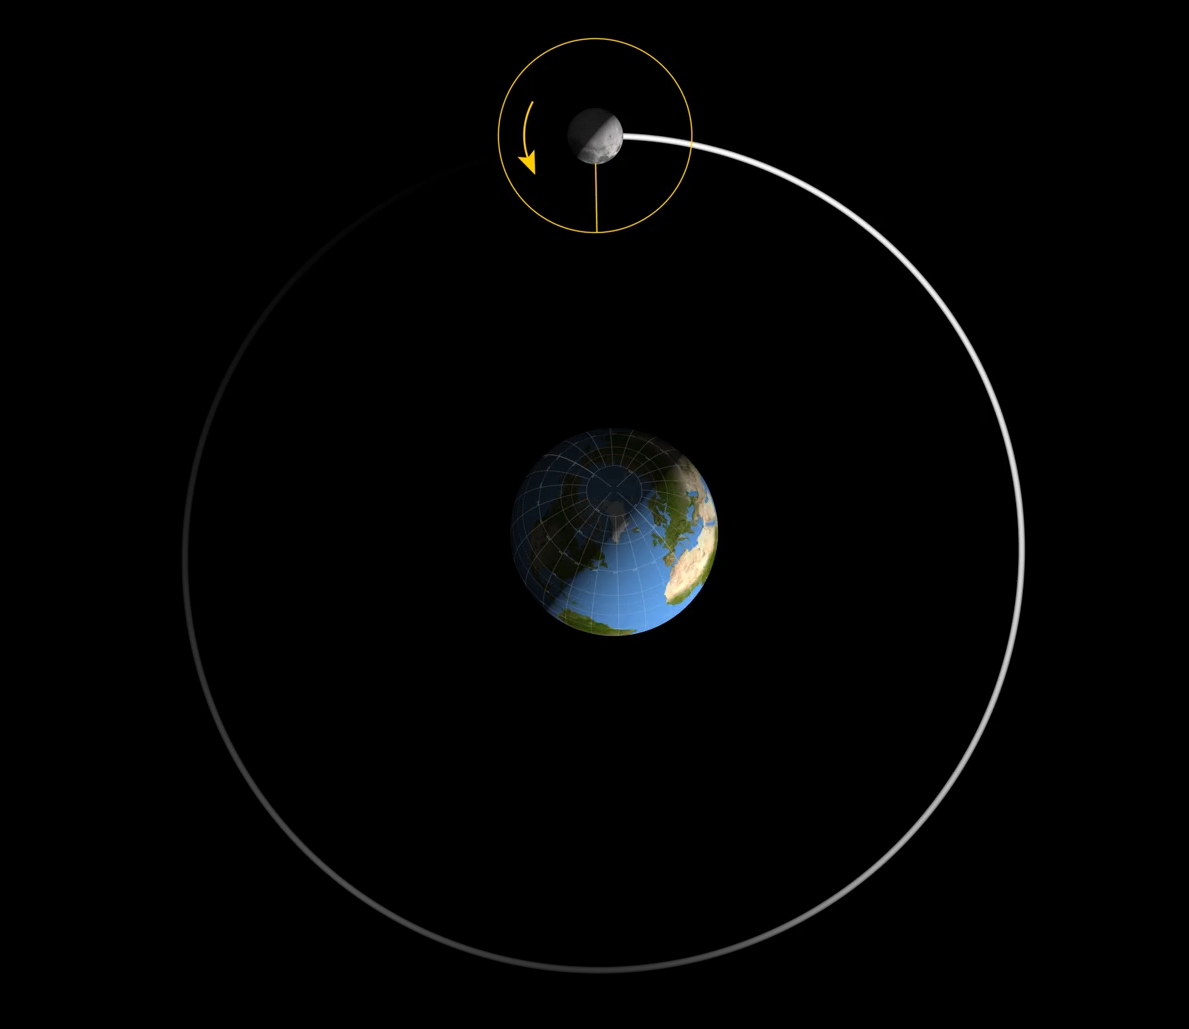
\includegraphics[width=0.7\textwidth]{MoonLocked.png}
    \caption{The Moon's rotation and orbit around the Earth, note that the shifting shadow of the Moon due to the Earth\cite{moonlock}}
    \label{fig:moon_rotation}
\end{figure}
\subsubsection{A Quick Aside to the Moon's Phases}
The Moon's phases depend on the relative positions of the Earth, Moon and Sun. The Moon's phases are a result of the changing angles between these three celestial bodies. The Moon's phases are as follows:
\begin{itemize}
    \item New Moon
    \item Waxing Crescent
    \item First Quarter
    \item Waxing Gibbous
    \item Full Moon
    \item Waning Gibbous
    \item Last Quarter
    \item Waning Crescent
\end{itemize}
\begin{figure}[H]
    \centering
    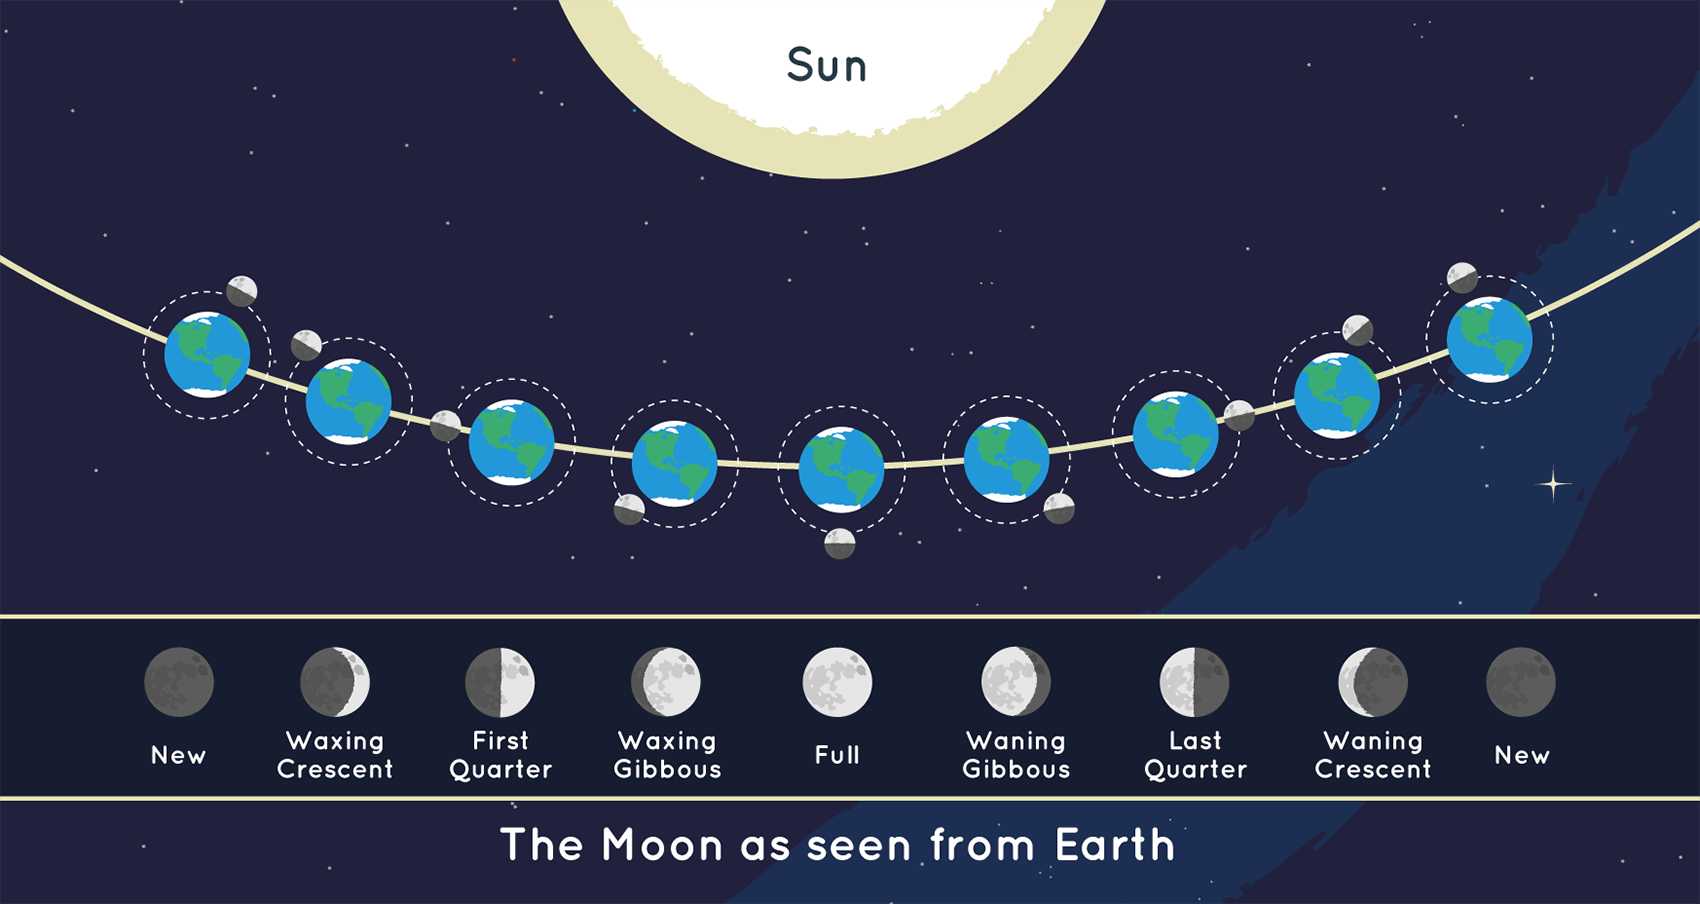
\includegraphics[width=0.7\textwidth]{moon-phases.en.png}
    \caption{The Moon's phases and their relative positions to the Earth and Sun\cite{moonphase}}
    \label{fig:moon_phases}
\end{figure}
Half of the Moon is always illuminated by the Sun, that is NOT always the side facing the Earth. When we see parts or none of the Moon illuminated, this is due to the angle of the Moon to the Sun, when the Moon is between the Earth and Sun, the lit half of the Moon is facing away from the Earth, this is called a New Moon. When the Moon is on the opposite side of the Earth from the Sun, the lit half of the Moon is facing the Earth, this is called a Full Moon. The other phases are a result of the Moon's position between these two extremes. What is important to remember is that the Moon's orbit is NOT in the same plane as the Earth's orbit of the sun, this means that the Moon's orbit is tilted at an angle of 5 degrees to the Earth's orbit, to explain why this occurs and what it means requires learning more on Lagrangian mechanics, elliptical orbits and the 3-body problem. None of which will be covered in depth, the reader is encouraged to look at textbooks and online resources to learn more about these topics.
\subsubsection{Finding the Moon's Rotational Angular Momentum}
What is known about the Moon is that it has a mass of \(m = 7.35 \times 10^{22} kg\) and a radius of \(r = 1.74 \times 10^6 m\). The time it takes the Moon to rotate around its own axis(or poles) is 29.5 days or 2548800 seconds, this is known as the synodic month. Meanwhile, the time it takes the Moon to orbit the Earth is 27.3 days, this is known as the sidereal month. For the Rotational Angular Momentum of the Moon, we will use the synodic month as the period of rotation. The angular momentum of the Moon can be calculated using the following equation:
\begin{equation}
    L = \frac{2}{5} m r^2 \cdot \frac{2 \pi}{T} = \frac{2}{5} (7.35 \times 10^{22} kg) (1.74 \times 10^6 m)^2 \cdot \frac{2 \pi}{2548800 s} = 2.194269 \times 10^{29} kg\cdot m^2/s
\end{equation}
While this number seems large, it is important to remember that the Moon is a massive object, and if we calculate the angular momentum of its orbit around the Earth, we will find that it is much larger than the angular momentum of the Moon's rotation. 
\section{Angular Momentum of The Moon's Orbit}
The Moon orbits the Earth, the orbital angular momentum is a slightly different than rotational. The moment of intertia for a body rotating around a point is:
\begin{equation}
    I=mr^2
\end{equation}
Using \ref{inertiaEQ} and \ref{angularMom}, with this new moment of intertia and different period, this is the lunar cycle, which is 27.3 days or 2358720 seconds. We can use the mean distance of 384,400 km, finally the orbital angular momentum is:
\begin{equation}
    L =  m_m r^2 \cdot \frac{2 \pi}{T} = (7.35 \times 10^{22} kg) (3.844 \times 10^8 m)^2 \cdot \frac{2 \pi}{2358720 s} = 2.88704309 \times 10^{34} kg\cdot m^2/s
\end{equation}
The Moon's orbital momentum is 100,000 times greater than the moons rotaional momentum.
\subsubsection{The Real Earth-Moon System}
The first section make some assumptions. First, the Moon and Earth are in a 2-body system. They both have angular and rotational momentum, the Moon and Earth cause tidal forces on each other. This results in "bulges" on the Moon and Earth. Momentum uses the SI unit $kg \cdot m^2/s$, this is literally built from the defintion of angular momentum in \ref{angGen}. There are so many assumptions to cover here, they descend from a 2 big assumptions:
\begin{itemize}
    \item The Moon is not in a circular orbit, it is in an elliptical orbit. This means that the Moon becomes closer and further from the Earth as it completes the orbit.
    \item The Moon's orbit is effected by the Earth's orbit around the sun, this system is actually a 3-body problem but the contribution is very small.
\end{itemize}
The Angular Momentum of the Moon is constant, but due to the Moon's elliptical orbit, its velocity and radius will change. With some mathematics and a few measurement techniques that scientist and astronauts put on the Moon half a century ago, we can measure the live distance from the Earth to the Moon.
\subsubsection{Measuring the Moon's Velocity and Distance}
In practical terms, the angular momentum of the Moon is mostly depending on the rotational, and the angular momentum the reader thinks about is the orbital momentum.
\begin{figure}[H]
    \centering
    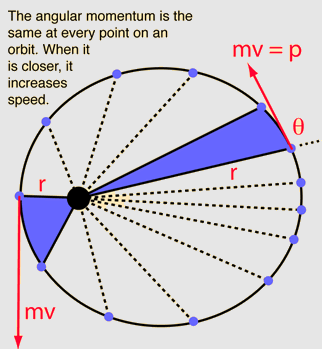
\includegraphics[width=0.5\textwidth]{VelocityVal.png}
    \caption{The Moon's speed will increase at the perigree and decrease as it approaches the apogee.}
\end{figure}
This will be the same as the angular momentum at the perigree and at the apogee. Using the Vis-Viva equation, the orbital speed of the moon:
\begin{equation}
    v = \sqrt{G(m_e+m_m)(\frac{2}{r}-\frac{1}{a})}
\end{equation}
$a$ is the length of the semi-major axis, this is simply the midpoint between the maximum and minimum radius: $\frac{r_{apogee}+r_{perigree}}{2}$. This means at any given point in the Moon's orbit, the reader can find the orbital velocity of the Moon. Using NASA's Earth Data's Normal Point Data Repository and API to access live LIDAR data for the distance the Moon is from the Earth \href{https://cddis.nasa.gov/Data_and_Derived_Products/SLR/Normal_point_data.html}{Normal Point Data}. The Apollo Missions left reflective mirrors on the Moon's surface so scientist today can using LIDAR to determine the distance, and is being updated daily by the International Laser Ranging Service(ILRS)\cite{LLR}. The reader should follow instructions at the database and register for API access, this document cannot cover specific instructions since the author cannot get access to the API at this time. If the reader wants to measure the speed of orbit, the reader can track the movement of the Moon in the sky using a telescope or astronomical tools; by measuring the angular displacement over a certain time to determine it's $\omega$.
\section{Moon's Magnetic Field}
The Moon has no magnetic field and but show deposits of magnetized metal deposits, scientist believes this shows the remnants of a magnetic field that may have once existed. This is an ongoing mystery that scientist are trying to solve.\cite{Moonfield} The reader can find surveys of the Moon's surface and magnetic field
\newpage
\section{References}
\bibliography{OrbitalMech.bib}
\bibliographystyle{ieeetr}
\end{document}


